\documentclass[12pt]{report}
\usepackage[utf8]{inputenc}
\usepackage[russian]{babel}
%\usepackage[14pt]{extsizes}
\usepackage{listings}
\usepackage{graphicx}
\usepackage{amsmath,amsfonts,amssymb,amsthm,mathtools} 
\usepackage{pgfplots}
\usepackage{filecontents}
\usepackage{float}
\usepackage{indentfirst}
\usepackage{eucal}
\usepackage{enumitem}
%s\documentclass[openany]{book}
\frenchspacing

\usepackage{indentfirst} % Красная строка

\usetikzlibrary{datavisualization}
\usetikzlibrary{datavisualization.formats.functions}

\usepackage{amsmath}


% Для листинга кода:
\lstset{ %
	language=c,                 % выбор языка для подсветки (здесь это С)
	basicstyle=\small\sffamily, % размер и начертание шрифта для подсветки кода
	numbers=left,               % где поставить нумерацию строк (слева\справа)
	numberstyle=\tiny,           % размер шрифта для номеров строк
	stepnumber=1,                   % размер шага между двумя номерами строк
	numbersep=5pt,                % как далеко отстоят номера строк от подсвечиваемого кода
	showspaces=false,            % показывать или нет пробелы специальными отступами
	showstringspaces=false,      % показывать или нет пробелы в строках
	showtabs=false,             % показывать или нет табуляцию в строках
	frame=single,              % рисовать рамку вокруг кода
	tabsize=2,                 % размер табуляции по умолчанию равен 2 пробелам
	captionpos=t,              % позиция заголовка вверху [t] или внизу [b] 
	breaklines=true,           % автоматически переносить строки (да\нет)
	breakatwhitespace=false, % переносить строки только если есть пробел
	escapeinside={\#*}{*)}   % если нужно добавить комментарии в коде
}


\usepackage[left=2cm,right=2cm, top=2cm,bottom=2cm,bindingoffset=0cm]{geometry}
% Для измененных титулов глав:
\usepackage{titlesec, blindtext, color} % подключаем нужные пакеты
\definecolor{gray75}{gray}{0.25} % определяем цвет
\newcommand{\hsp}{\hspace{20pt}} % длина линии в 20pt
% titleformat определяет стиль
\titleformat{\chapter}[hang]{\Huge\bfseries}{\thechapter\hsp\textcolor{gray75}{|}\hsp}{0pt}{\Huge\bfseries}


% plot
\usepackage{pgfplots}
\usepackage{filecontents}
\usetikzlibrary{datavisualization}
\usetikzlibrary{datavisualization.formats.functions}

\begin{document}

\begin{titlepage}
	\newgeometry{pdftex, left=2cm, right=2cm, top=2.5cm, bottom=2.5cm}
	\fontsize{12pt}{12pt}\selectfont
	\noindent \begin{minipage}{0.15\textwidth}
		
\includegraphics[width=\linewidth]{pictures/b_logo.jpg}
	\end{minipage}
	\noindent\begin{minipage}{0.9\textwidth}\centering
		\textbf{Министерство науки и высшего образования Российской Федерации}\\
		\textbf{Федеральное государственное бюджетное образовательное учреждение высшего образования}\\
		\textbf{«Московский государственный технический университет имени Н.Э.~Баумана}\\
		\textbf{(национальный исследовательский университет)»}\\
		\textbf{(МГТУ им. Н.Э.~Баумана)}
	\end{minipage}
	
	\noindent\rule{18cm}{3pt}
	\newline\newline
	\noindent ФАКУЛЬТЕТ $\underline{\text{«Информатика и системы управления»}}$ \newline\newline
	\noindent КАФЕДРА $\underline{\text{«Программное обеспечение ЭВМ и информационные технологии»}}$\newline\newline\newline\newline\newline\newline\newline
	
	
	\begin{center}
		\Large\textbf{Отчет по лабораторной работе №4}\newline
	\end{center}
	
	\noindent\textbf{Название} $\underline{\text{~Моделирование системы массового обслуживания~~~~~~~~~}}$\newline\newline\newline
	\noindent\textbf{Дисциплина} $\underline{\text{~Моделирование~~~~~~~~}}$\newline\newline
	\noindent\textbf{Студент} $\underline{\text{Золотухин А. В.~~~~~~~~~~~~~~~~~~~~~~~~~~~~~~~~~~~~~~~~~}}$\newline\newline
	\noindent\textbf{Группа} $\underline{\text{ИУ7-74Б~~~~~~~~~~~~~~~~~~~~~~~~~~~~~~~~~~~~~~~~~~~~}}$\newline\newline
	\noindent\textbf{Оценка (баллы)} $\underline{\text{~~~~~~~~~~~~~~~~~~~~~~~~~~~~~~~~~~~~~~~~~~~~~~~~~}}$\newline\newline
	\noindent\textbf{Преподаватель}$\underline{\text{~Рудаков И. В.~~~~~~~~~~}}$\newline
	
	\begin{center}
		\vfill
		Москва~---~\the\year
		~г.
	\end{center}
 \restoregeometry
\end{titlepage}


\chapter{Задание}

\section{Цель работы}

\textbf{Цель работы:} построение доверительных интервалов для математического ожидания и дисперсии нормальной случайной величины.

\section{Содержание работы}

\begin{enumerate}
    \item Для выборки объема $n$ из нормальной генеральной совокупности $X$ реализовать в виде программы на ЭВМ
        \begin{enumerate}
            \item вычисление точечных оценок $\hat\mu(\vec x_n)$ и $S^2(\vec x_n)$ математического ожидания $MX$ и дисперсии $DX$ соответственно;
            \item вычисление нижней и верхней границ $\underline\mu(\vec x_n)$, $\overline\mu(\vec x_n)$ для $\gamma$-доверительного интервала для математического ожидания $MX$;
            \item вычисление нижней и верхней границ $\underline\sigma^2(\vec x_n)$, $\overline\sigma^2(\vec x_n)$ для $\gamma$-доверительного интервала для дисперсии $DX$;
        \end{enumerate}
    \item вычислить $\hat\mu$ и $S^2$ для выборки из индивидуального варианта;
    \item для заданного пользователем уровня доверия $\gamma$ и $N$ – объёма выборки из индивидуального варианта:
        \begin{enumerate}
            \item на координатной плоскости $Oyn$ построить прямую $y = \hat\mu(\vec{x_N})$, также графики функций $y = \hat\mu(\vec x_n)$, $y = \underline\mu(\vec x_n)$ и $y = \overline\mu(\vec x_n)$ как функций объема $n$ выборки, где $n$ изменяется от 1 до $N$;
            \item на другой координатной плоскости $Ozn$ построить прямую $z = S^2(\vec{x_N})$, также графики функций $z = S^2(\vec x_n)$, $z = \underline\sigma^2(\vec x_n)$ и $z = \overline\sigma^2(\vec x_n)$ как функций объема $n$ выборки, где $n$ изменяется от 1 до $N$.
        \end{enumerate}
\end{enumerate}

\chapter{Теоретическая часть}

\section{Определение $\gamma$-доверительного интервала для значения параметра распределения случайной величины}

Пусть $X$ --- случайная величина, закон распределения которой зависит от вектора $\vec \theta = (\theta_{1}, ..., \theta_{r})$ неизвестных параметров. Будем считать, что $r = 1$, т. е. $\vec \theta = (\theta_{1}) = (\theta)$.

\underline{Опр.} Интервальной оценкой параметра $\theta$ уровня $\gamma$ ($\gamma$-интервальной оценкой) называют пару статистик $\underline{\theta}(\vec X)$ и $\overline{\theta}(\vec X)$ таких, что
\begin{equation}
	P\{\theta \in (\underline{\theta}(\vec X), \overline{\theta}(\vec X)\} = \gamma, \gamma \in (0;1).
\end{equation}

\underline{Опр.} $\gamma$-доверительным интервалом (доверительным интервалом уровня $\gamma$) для параметра $\theta$ называют реализацию (выборочное значение) интервальной оценкой уровня $\gamma$ для этого параметра, т.е. интервал $(\underline{\theta}(\vec x), \overline{\theta}(\vec x))$ с детерминированными границами.

\section{Формулы для вычисления границ \newline$\gamma$-доверительного интервала для математического ожидания и дисперсии нормальной случайной величины}

Пусть $N(\mu, \sigma^2)$ --- общий вид закона распределения генеральной совокупности $X$. $\mu$, $\sigma^2$ --- неизвестны. 

Границы $\gamma$-доверительного интервала для математического ожидания нормальной случайной величины:
\begin{equation}
	\underline{\mu}(\vec x) = \overline{x} - \frac{S(\vec x)t^{(n - 1)}_{\frac{1 + \gamma}{2}}}{\sqrt{n}},
\end{equation}
\begin{equation}
	\overline{\mu}(\vec x) = \overline{x} + \frac{S(\vec x)t^{(n - 1)}_{\frac{1 + \gamma}{2}}}{\sqrt{n}},
\end{equation}
где $\overline{x} = \frac{1}{n} \sum_{i=1}^n x_i$; $S(\vec x) = \sqrt{\frac{1}{n-1} \sum_{i=1}^n (x_i - \overline x)^2}$; $t^{(n - 1)}_{\frac{1 + \gamma}{2}}$ --- квантиль уровня $\frac{1 + \gamma}{2}$ распределения Стьюдента с $n - 1$ степенями свободы; $n$ --- объем выборки.

Границы $\gamma$-доверительного интервала для дисперсии нормальной случайной величины:

\begin{equation}
	\underline{\sigma}^2(\vec x) = \frac{(n - 1)S^2(\vec x)}{h^{(n - 1)}_{\frac{1 + \gamma}{2}}},
\end{equation}
\begin{equation}
	\overline{\sigma}^2(\vec x) = \frac{(n - 1)S^2(\vec x)}{h^{(n - 1)}_{\frac{1 - \gamma}{2}}},
\end{equation}
где $n$ --- объем выборки; $S^2(\vec x) = \frac{1}{n-1} \sum_{i=1}^n (x_i - \overline x)^2$; $h^{(n - 1)}_{\frac{1 + \gamma}{2}}$, $h^{(n - 1)}_{\frac{1 - \gamma}{2}}$ --- квантили уровня $\frac{1 + \gamma}{2}$ и $\frac{1 - \gamma}{2}$ соответственно распределения $\chi^2(n - 1)$.

\chapter{Практическая часть}

\begin{lstlisting}[language=Matlab]
gamma = 0.9;
n = length(X);

% 1
mu = expectation(X);
s2 = variance(X);
fprintf('mu = %.2f\n', mu); 
fprintf('S^2 = %.2f\n\n', s2);

mu_low = mu + (sqrt(s2) * tinv((1 - gamma) / 2, n - 1)) / sqrt(n);
mu_high = mu + (sqrt(s2) * tinv((1 + gamma) / 2, n - 1)) / sqrt(n);
fprintf('mu_low = %.2f\n', mu_low);
fprintf('mu_high = %.2f\n\n', mu_high);

sigma_low  = ((n - 1) * s2) / chi2inv((1 + gamma) / 2, n - 1);
sigma_high = ((n - 1) * s2) / chi2inv((1 - gamma) / 2, n - 1);
fprintf('sigma_low = %.2f\n', sigma_low);
fprintf('sigma_high = %.2f\n\n', sigma_high);

MX = mean(X);
DX = var(X);
fprintf("MX = %.2f\n", MX);   
fprintf("DX = %.2f\n", DX);

% 3
n_array = zeros([1 n]);
mu_array = zeros([1 n]);
mu_low_array = zeros([1 n]);
mu_high_array = zeros([1 n]);
s2_array = zeros([1 n]);
s2_low_array = zeros([1 n]);
s2_high_array = zeros([1 n]);

for i = 1:n
	n_array(i) = i;

mu_i = find_mu(X(1:i));
mu_array(i) = mu_i;
s_sqr_i = find_s_sqr(X(1:i));
s2_array(i) = s_sqr_i;

mu_low_array(i) = find_mu_low(mu_i, s_sqr_i, i, gamma);
mu_high_array(i) = find_mu_high(mu_i, s_sqr_i, i, gamma);

s2_low_array(i) = find_sigma_sqr_low(s_sqr_i, i, gamma);
s2_high_array(i) = find_sigma_sqr_high(s_sqr_i, i, gamma);
end

mu_const = mu * ones(n);
s2_const = s2 * ones(n);

% a
plot(n_array, mu_const, n_array, mu_array, ...
n_array, mu_low_array, n_array, mu_high_array);
xlabel('n');
ylabel('y');
xlim([10 n]);
legend('$\hat \mu(\vec x_N)$', '$\hat \mu(\vec x_n)$', ...
'$\underline{\mu}(\vec x_n)$', '$\overline{\mu}(\vec x_n)$', ...
'Interpreter', 'latex', 'FontSize', 14);
figure;

% b
plot(n_array, s2_const, n_array, s2_array, ...
n_array, s2_low_array, n_array, s2_high_array);
xlabel('n');
ylabel('z');
xlim([10 n]);
legend('$\hat S^2(\vec x_N)$', '$\hat S^2(\vec x_n)$', ...
'$\underline{\sigma}^2(\vec x_n)$', '$\overline{\sigma}^2(\vec x_n)$', ...
'Interpreter', 'latex', 'FontSize', 14);

% Help functions
function [mu] = find_mu(X)
	mu = mean(X);
end

function [s_sqr] = find_s_sqr(X)
	s_sqr = var(X);
end

function [mu_low] = find_mu_low(mu, s_sqr, n, gamma)
	mu_low = mu - sqrt(s_sqr) * tinv((1 + gamma) / 2, n - 1) / sqrt(n);
end

function [mu_high] = find_mu_high(mu, s_sqr, n, gamma)
	mu_high = mu + sqrt(s_sqr) * tinv((1 + gamma) / 2, n - 1) / sqrt(n);
end

function [sigma_sqr_low] = find_sigma_sqr_low(s_sqr, n, gamma)
	sigma_sqr_low = (n - 1) * s_sqr / chi2inv((1 + gamma) / 2, n - 1);
end

function [sigma_sqr_high] = find_sigma_sqr_high(s_sqr, n, gamma)
	sigma_sqr_high = (n - 1) * s_sqr / chi2inv((1 - gamma) / 2, n - 1);
end

function mu = expectation(x)
	mu = sum(x) / length(x);
end

function s2 = variance(x)
	n = length(x);
	mu = expectation(x);
	s2 = sum((x - mu).^2) / (n - 1);
end
\end{lstlisting}


\chapter{Экспериментальная часть}

\section{Результаты расчетов}

Выборка:
$\vec x$=[3.89,2.60,2.56,2.33,4.35,3.97,4.16,4.10,4.82,3.17,4.15,4.05,4.45,3.76,4.83,4.27,2.03,3.13,\\3.69,5.44,2.61,5.20,4.03,5.26,4.42,3.67,4.68,5.22,4.11,3.35,3.83,5.34,4.69,5.12,4.33,4.41,4.82,4.65,3.12,4.71,\\2.36,3.10,3.52,1.74,3.46,2.89,5.42,4.12,5.36,4.26,3.49,5.85,5.24,4.23,4.57,3.54,4.38,4.31,2.28,4.17,3.66,5.25,\\3.11,4.48,3.80,4.05,3.48,1.12,2.16,4.68,4.21,3.22,4.29,4.70,4.37,4.60,4.15,4.06,3.81,3.58,4.34,3.87,4.53,6.02,\\3.34,3.34,2.87,4.64,3.03,3.08,3.46,4.04,4.77,3.59,3.49,6.53,4.16,2.95,4.85,5.53,3.59,4.24,4.45,4.42,4.10,3.77,\\4.56,3.89,4.13,4.00,3.95,2.73,4.76,3.19,3.66,4.87,4.18,5.30,4.97,4.56];

Результаты работы программы для выборки (Вариант 4) представлены на рисунках \ref{fig2}, \ref{fig3}.

\begin{equation*}
    \hat\mu(\vec x_n) = 4.03\\
\end{equation*}
\begin{equation*}
    S^2(\vec x_n) = 0.83\\
\end{equation*}
\begin{equation*}
    \underline\mu(\vec x_n) = 3.90\\
\end{equation*}
\begin{equation*}
    \overline\mu(\vec x_n) =  4.17\\
\end{equation*}
\begin{equation*}
    \underline{S^2}(\vec x_n) = 0.68\\
\end{equation*}
\begin{equation*}
    \overline{S^2}(\vec x_n) = 1.04\\
\end{equation*}


\begin{figure}[ht!]	
	\centering{
		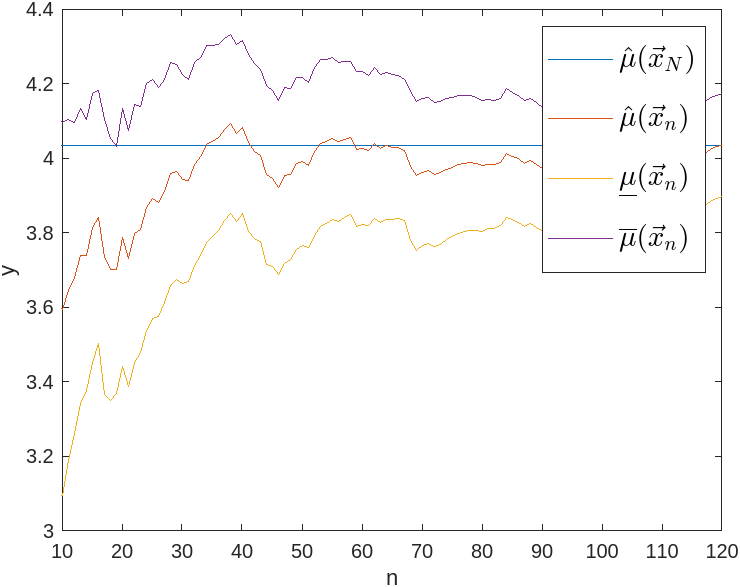
\includegraphics[width=0.7\textwidth]{res1}
		\caption{Прямая $y(n) = \hat\mu(\vec x_N)$, а также графики функций  $y(n) = \hat\mu(\vec x_n)$, $y(n) = \underline\mu(\vec x_n)$, $y(n) = \overline\mu(\vec x_n)$ как функций объема $n$ выборки, где $n$ изменяется от 10 до $N$}
	\label{fig2}}
\end{figure}


\begin{figure}[ht!]	
	\centering{
		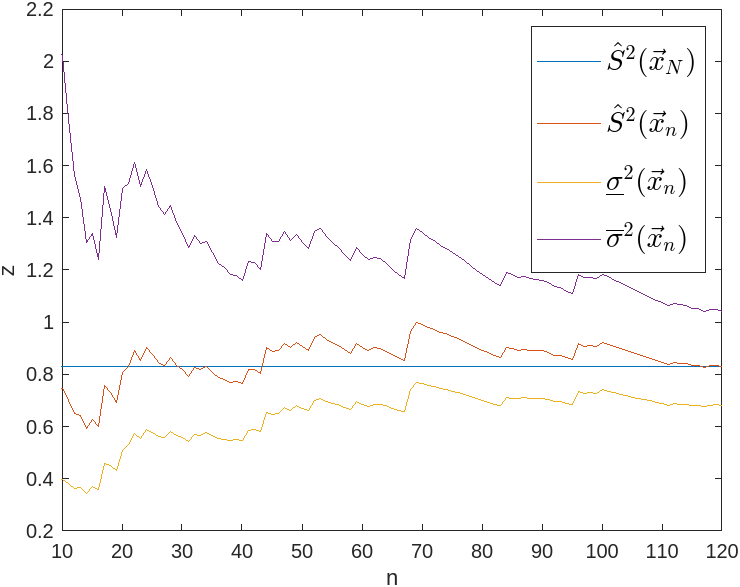
\includegraphics[width=0.7\textwidth]{res2}
		\caption{Прямая $z(n) = \hat S^2(\vec x_N)$, а также графики функций $z(n) = \hat S^2(\vec x_n)$, $z(n) = \underline \sigma^2(\vec x_n)$, $z(n) = \overline \sigma^2(\vec x_n)$ как функций объема $n$ выборки, где $n$ изменяется от 10 до $N$}
	\label{fig3}}
\end{figure}


\end{document}
